%========================================
\chapter{Design Document}
%========================================

\section{System Architecture}

AgriQueue is architected as a modular, three-tier cloud platform designed for scalability, low latency, and fault tolerance:
\begin{itemize}
  \item \textbf{Tier 1 -- Presentation Layer:} React 19 Single Page Application (SPA) deployed across globally distributed edge nodes on Vercel CDN. Supports responsive views tailored for farmers (mobile-first), staff (operational dashboard), and administrators (analytics portal).
  \item \textbf{Tier 2 -- Application Layer:} FastAPI asynchronous ASGI web server running on Uvicorn workers. Houses authentication guards, the slot capacity engine, the real-time SSE queue broadcaster, the scikit-learn ML inference pipeline, and the LangGraph-powered AI assistant.
  \item \textbf{Tier 3 -- Persistence \& External Services:} Managed PostgreSQL 15 database accessed via SQLAlchemy 2.0 async ORM and the high-throughput \texttt{asyncpg} driver, alongside VAPID Web Push servers and Google Gemini LLM cloud infrastructure.
\end{itemize}

\begin{figure}[H]
\centering
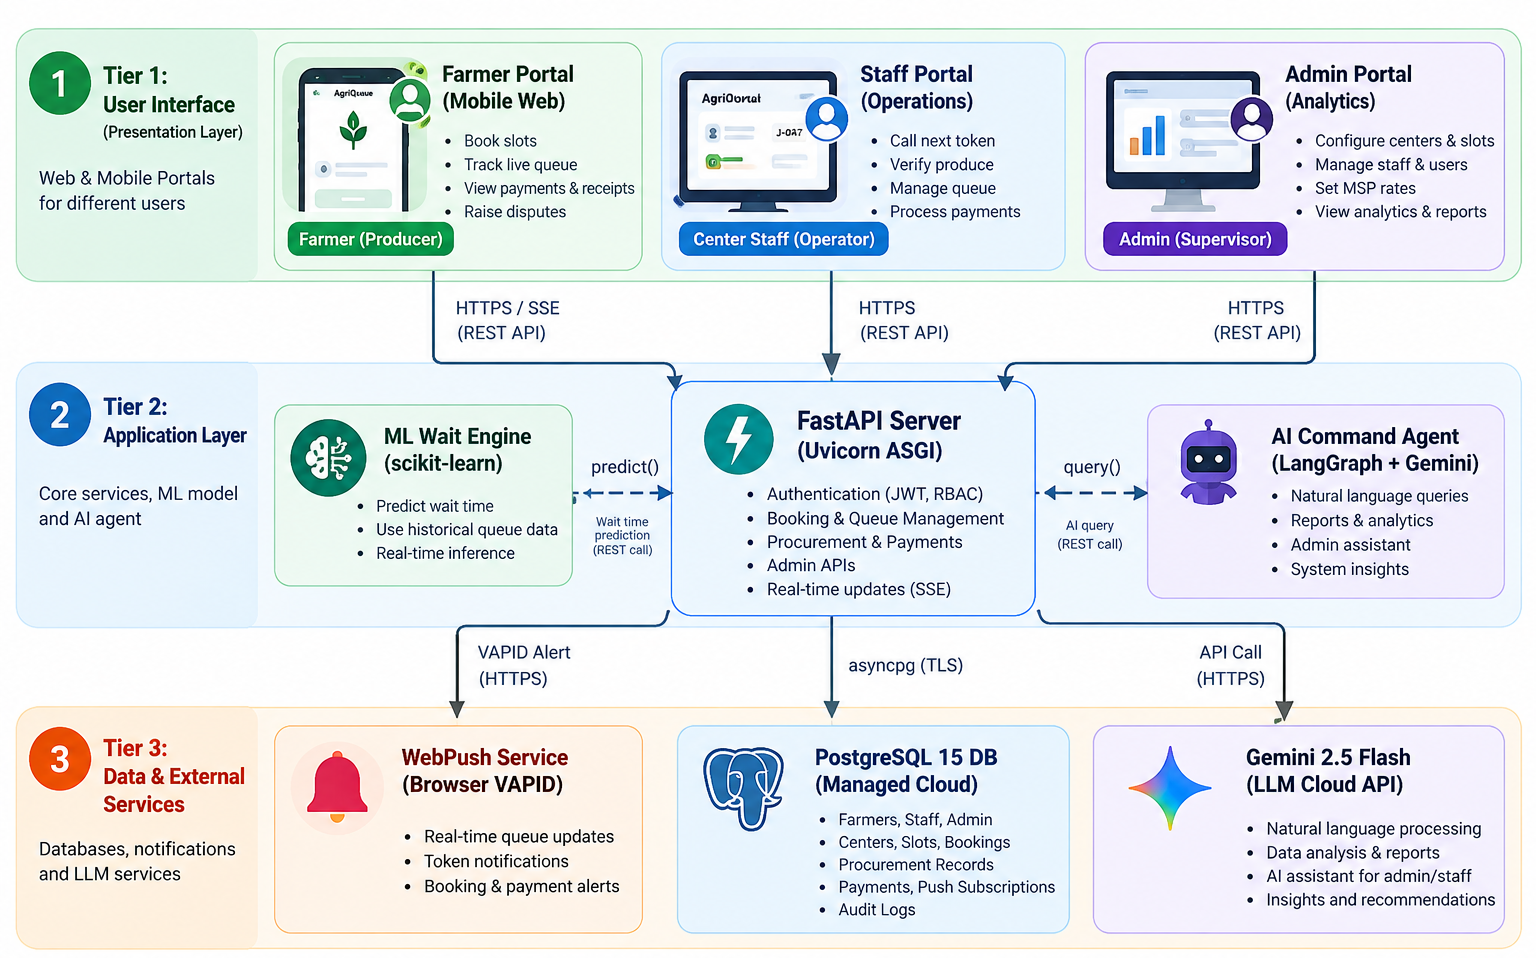
\includegraphics[width=\textwidth]{img/three_tier_clean.png}
\caption{AgriQueue Three-Tier Modular System Architecture}
\label{fig:arch}
\end{figure}

\begin{itemize}
  \item \textbf{Presentation Tier:} Delivers single-page responsive user interfaces rendered entirely on client devices with client-side routing via React Router.
  \item \textbf{Application Tier:} Stateless RESTful API server handling request validation (Pydantic), token parsing (JWT), queue sequencing, and ML wait time estimation.
  \item \textbf{Data Tier:} ACID-compliant relational data store with indexed queries for sub-10ms response times on active queues and booking verification.
\end{itemize}

\section{System Use Cases}

\begin{table}[H]
\centering
\caption{Detailed System Use Cases by Role}
\label{tab:usecases}
\renewcommand{\arraystretch}{1.2}
\begin{tabular}{|p{2.2cm}|p{3.5cm}|p{7.8cm}|}
\hline
\textbf{Role} & \textbf{Category} & \textbf{Key Use Cases} \\ \hline
\multirow{4}{*}{\textbf{Farmer}} 
  & Account & Register account, Login via JWT cookie, View profile, Logout \\ \cline{2-3}
  & Booking & Search centers, View slot capacity, Book slot, Cancel booking \\ \cline{2-3}
  & Live Queue & Stream live token queue via SSE, Track estimated wait time \\ \cline{2-3}
  & Finance & View procurement receipt, Track payment status, Raise dispute \\ \hline
\multirow{3}{*}{\textbf{Staff}} 
  & Queue Mgmt & View daily center queue, Call next token, Mark farmer serving \\ \cline{2-3}
  & Procurement & Weigh produce, Enter moisture \& deductions, Compute payable \\ \cline{2-3}
  & Payments & Complete procurement, Initiate payment, Resolve farmer disputes \\ \hline
\multirow{3}{*}{\textbf{Admin}} 
  & Center Mgmt & Add/edit procurement centers, Configure time slots \& capacity \\ \cline{2-3}
  & Pricing & Set government MSP rates per produce and quality grade \\ \cline{2-3}
  & Staff \& Audit & Register staff accounts, Assign centers, Monitor system analytics \\ \hline
\end{tabular}
\end{table}

\section{Data Flow Diagrams (DFD)}

Data Flow Diagrams model the flow of data through the AgriQueue platform, detailing transformations across system processes, operational actors, and persistent datastores.

\subsection{DFD Level 0: Context-Level Diagram}

The Context Diagram defines the external boundary of the platform, illustrating key inputs and outputs between AgriQueue and the primary external entities:

\begin{figure}[H]
\centering
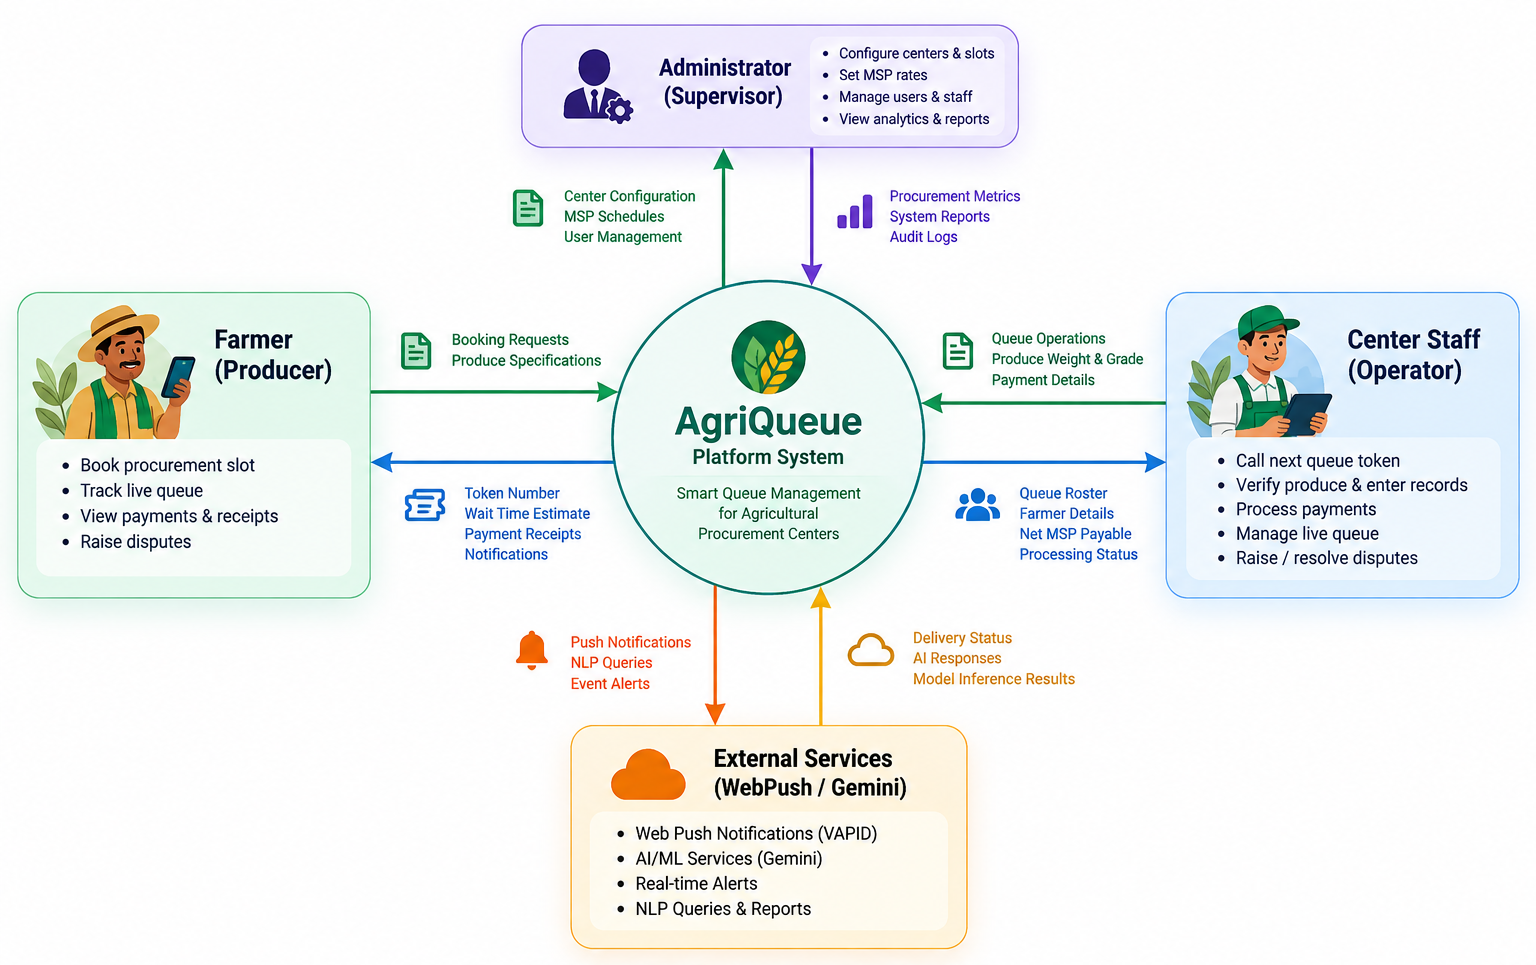
\includegraphics[width=\textwidth]{img/dfd_l0_clean.png}
\caption{DFD Level 0: AgriQueue Context-Level Data Flow Diagram}
\label{fig:dfd0}
\end{figure}

\newpage
\subsection{DFD Level 1: Subsystem Data Flow Decomposition}

The Level 1 DFD decomposes the central system into seven functional processes and five persistent datastores:

\definecolor{procfill}{RGB}{218, 238, 255}
\definecolor{procborder}{RGB}{24, 110, 185}
\definecolor{entfill}{RGB}{230, 218, 255}
\definecolor{entborder}{RGB}{100, 45, 175}
\definecolor{dstorefill}{RGB}{255, 226, 192}
\definecolor{dstoreborder}{RGB}{215, 105, 25}

\begin{figure}[H]
\centering
\resizebox{\textwidth}{!}{%
\begin{tikzpicture}[
  proc/.style={
    rectangle, draw=procborder, fill=procfill, rounded corners=6pt,
    text width=2.9cm, minimum height=1.25cm, align=center,
    font=\fontsize{9pt}{11pt}\selectfont\bfseries, line width=0.9pt
  },
  ent/.style={
    rectangle, draw=entborder, fill=entfill, rounded corners=6pt,
    text width=2.6cm, minimum height=1.15cm, align=center,
    font=\fontsize{9pt}{11pt}\selectfont\bfseries, line width=0.9pt
  },
  dstore/.style={
    cylinder, shape border rotate=90, aspect=0.25,
    draw=dstoreborder, fill=dstorefill,
    text width=2.7cm, minimum height=1.15cm, align=center,
    font=\fontsize{9pt}{11pt}\selectfont\bfseries, line width=0.9pt
  },
  arr/.style={->, >=Latex, line width=0.75pt, draw=black!90},
  darr/.style={<->, >=Latex, line width=0.75pt, draw=black!90},
  dasharr/.style={->, >=Latex, dashed, line width=0.75pt, draw=black!90},
  lbl/.style={fill=white, inner sep=1.2pt, font=\fontsize{7.5pt}{9pt}\selectfont, align=center}
]

% Diagram Title (Top Centered)
\node[font=\LARGE\bfseries] at (7.4, 10.0) {AgriQueue -- Level 1 Data Flow Diagram};

% --- NODES ---
% Row Top (y = 8.4): D1 and Administrator
\node[dstore] (D1) at (3.6, 8.4) {D1: Users \&\\Credentials};
\node[ent] (E_ADM) at (8.6, 8.4) {Administrator\\(Supervisor)};

% Row 1 (y = 5.6): Process 1.0, Process 2.0, Datastore D2
\node[proc] (P1) at (3.6, 5.6) {1.0\\Authentication\\\& RBAC};
\node[proc] (P2) at (8.6, 5.6) {2.0\\Slot Capacity\\\& Schedules};
\node[dstore] (D2) at (15.8, 5.6) {D2: Centers,\\Slots \& Rates};

% Farmer Entity (y = 5.6)
\node[ent] (E_FAR) at (-1.5, 5.6) {Farmer\\(Producer)};

% Row 2 (y = 2.4): Process 3.0, Process 4.0, Process 5.0
\node[proc] (P3) at (3.6, 2.4) {3.0\\Booking \&\\Token Engine};
\node[proc] (P4) at (8.6, 2.4) {4.0\\ML Wait-Time\\Inference};
\node[proc] (P5) at (13.8, 2.4) {5.0\\Live SSE\\Queue Stream};

% Row 3: Datastore D3 (y = 0.3), Process 6.0 (y = -1.6), Datastore D4 (y = -1.6)
\node[dstore] (D3) at (3.6, 0.3) {D3: Active\\Queue Tokens};
\node[proc] (P6) at (9.4, -1.6) {6.0\\Weighing\\Verification};
\node[dstore] (D4) at (15.8, -1.6) {D4: Scale Records};

% Row 4 (y = -4.0): Datastore D5, Process 7.0, Entity Center Staff
\node[dstore] (D5) at (2.2, -4.0) {D5: Payments\\\& Receipts};
\node[proc] (P7) at (8.0, -4.0) {7.0\\Payment\\Settlement};
\node[ent] (E_STA) at (13.2, -4.0) {Center Staff\\(Operator)};

% --- FLOWS / ARROWS ---

% 1. Farmer <-> P1
\draw[arr] ([yshift=7pt]E_FAR.east) -- ([yshift=7pt]P1.west)
  node[midway, lbl, above=1pt]{Login Request};
\draw[arr] ([yshift=-7pt]P1.west) -- ([yshift=-7pt]E_FAR.east)
  node[midway, lbl, below=1pt]{(authenticated)};

% 2. P1 <-> D1
\draw[darr] (P1.north) -- (D1.south)
  node[midway, lbl, right=3pt]{Verify / Read};

% 3. Admin -> P2
\draw[arr] (E_ADM.south) -- (P2.north)
  node[midway, lbl, right=3pt]{Slot Quotas};

% 4. P2 <-> D2
\draw[arr] ([yshift=7pt]P2.east) -- ([yshift=7pt]D2.west)
  node[midway, lbl, above=1pt]{Update Slots};
\draw[arr] ([yshift=-7pt]D2.west) -- ([yshift=-7pt]P2.east)
  node[midway, lbl, below=1pt]{Center Baseline};

% 5. P2 -> P3 (Capacity OK)
\draw[arr] ([xshift=-16pt]P2.south) -- ++(0, -1.0) -| (P3.north);
\node[lbl] at (6.8, 4.3) {Capacity OK};

% 6. Farmer Bus & Connections
% Bus dropping from Farmer bottom-center
\coordinate (FAR_BUS) at ([xshift=2pt]E_FAR.south);
\coordinate (FAR_BUS_END) at ([xshift=2pt]E_FAR.south |- 0, -2.5);
\draw[line width=0.75pt, draw=black!90] (FAR_BUS) -- (FAR_BUS_END);

% Book Slot (from Farmer bottom-right)
\draw[arr] ([xshift=18pt]E_FAR.south) |- ([yshift=10pt]P3.west)
  node[pos=0.75, lbl, above=1pt]{Book Slot};

% Token Card (from P3 west to FAR_BUS)
\draw[arr] ([yshift=-8pt]P3.west) -- ([yshift=-8pt]P3.west -| FAR_BUS)
  node[midway, lbl, below=1pt]{Token Card};

% 7. P3 -> P4 (Queue Features)
\draw[arr] (P3.east) -- (P4.west)
  node[midway, lbl, above=1pt]{Queue\\Features};

% 8. P4 -> P5 (Wait Estimate)
\draw[arr] (P4.east) -- (P5.west)
  node[midway, lbl, above=1pt]{Wait\\Estimate};

% 9. D2 -> P4 (Center Baseline / Rates)
\draw[arr] ([xshift=-16pt]D2.south) -- ++(0, -1.2) -| (P4.north)
  node[pos=0.45, lbl, below=1pt]{Center Baseline / Rates};

% 10. D2 -> P6 (MSP Rates)
\draw[arr] ([xshift=12pt]D2.south) -- ++(0, -5.2) -| ([xshift=14pt]P6.north);
\node[lbl, above=1pt] at (12.8, -0.65) {MSP Rates};

% 11. P3 <-> D3 (Commit Token & Active Queue)
\draw[arr] ([xshift=-12pt]P3.south) -- ([xshift=-12pt]D3.north)
  node[midway, lbl, left=2pt]{Commit Token};
\draw[arr] ([xshift=12pt]D3.north) -- ([xshift=12pt]P3.south)
  node[midway, lbl, right=2pt]{Active Queue};

% 12. D3 <-> P5
% Active Queue (read): from 5.0 south, down to y=0.5, then left into D3 east
\draw[arr] ([xshift=-16pt]P5.south) |- ([yshift=6pt]D3.east)
  node[pos=0.68, lbl, above=1pt]{Active Queue (read)};
% Active Queue Updates: from D3 east, horizontally right at y=0.1 to x=14.2, then up to 5.0 south
\draw[arr] ([yshift=-6pt]D3.east) -| ([xshift=10pt]P5.south)
  node[pos=0.38, lbl, above=1pt]{Active Queue Updates};

% 13. P3 -> P6 (Dashed: Completed Booking for processing)
\draw[dasharr] ([yshift=-12pt]P3.east) -- ++(1.4, 0) |- ([yshift=3pt]P6.west);
\node[lbl] at (6.6, -1.0) {Completed Booking\\(for processing)};

% 14. 5.0 -> 6.0 & Farmer (SSE Queue Stream)
% Branch into 6.0
\draw[arr] ([xshift=-4pt]P5.south) -- ++(0, -2.6) -| ([xshift=-6pt]P6.north);
% Long stream to Farmer Bus (horizontal at y = -2.5)
\draw[arr] ([xshift=-4pt]P5.south) -- ([xshift=-4pt]P5.south |- 0, -2.5) -- (FAR_BUS_END);
\node[lbl, above=1pt] at (3.6, -2.4) {SSE Queue Stream (live updates)};

% 15. P6 -> D4 (Save Scales)
\draw[arr] (P6.east) -- (D4.west)
  node[midway, lbl, above=1pt]{Save Scales};

% 16. Center Staff -> P6 (Gross Wt, Deductions)
\draw[arr] (E_STA.north) |- ([yshift=-8pt]P6.east)
  node[pos=0.35, lbl, left=4pt]{Gross Wt, Deductions};

% 17. P6 -> P7 (Net Payable - strictly vertical)
\draw[arr] (8.5, -2.225) -- (8.5, -3.375)
  node[midway, lbl, right=3pt]{Net Payable};

% 18. P7 -> D5 (Disburse / Payment Record)
\draw[arr] (P7.west) -- (D5.east)
  node[midway, lbl, above=1pt]{Disburse /\\Payment Record};

% 19. D5 -> Farmer (Digital Receipt)
\draw[arr] (D5.west) -| ([xshift=-22pt]E_FAR.south)
  node[pos=0.22, lbl, above=1pt]{Digital Receipt};

\end{tikzpicture}%
}
\caption{DFD Level 1: Subsystem Process Decomposition and Data Stores}
\label{fig:dfd1}
\end{figure}

\newpage
\section{Entity Relationship Model}

The relational data model comprises 12 entities structured to maintain referential integrity across the booking and payment lifecycle:

\begin{figure}[H]
\centering
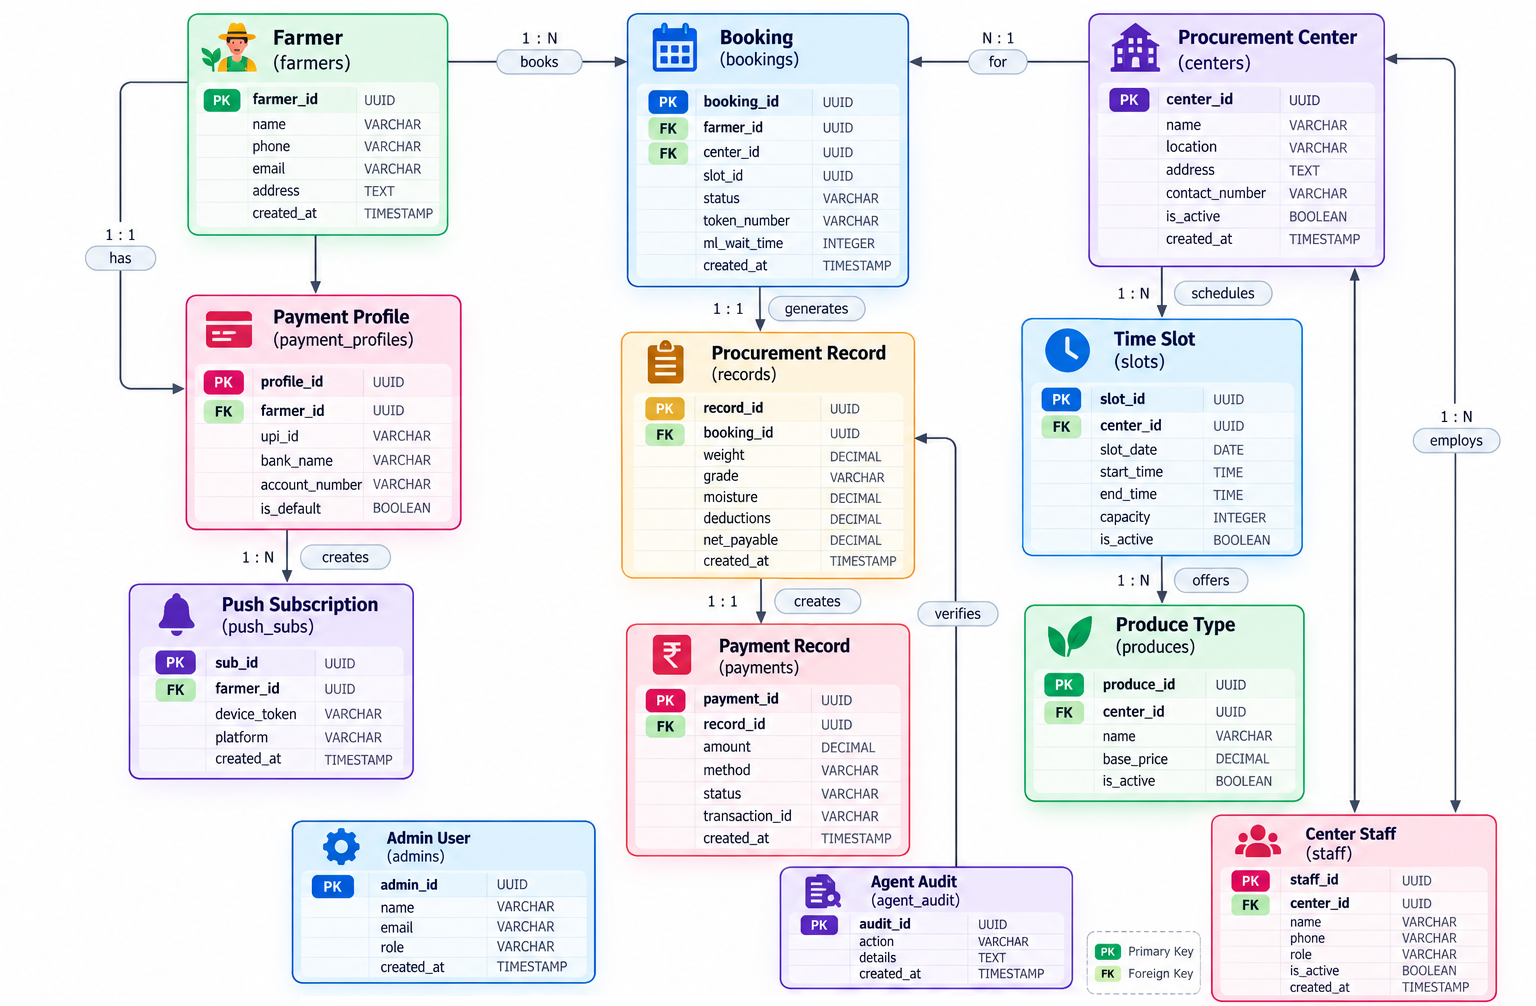
\includegraphics[width=\textwidth]{img/erd_clean.png}
\caption{AgriQueue Relational Entity Relationship Diagram}
\label{fig:erd}
\end{figure}

\begin{itemize}
  \item \textbf{Farmer to Booking (1:N):} A registered farmer can schedule multiple procurement bookings across different dates and seasons.
  \item \textbf{Center to Slot and Booking (1:N):} Centers partition daily operational hours into distinct slots, each enforcing an independent capacity ceiling.
  \item \textbf{Booking to Procurement Record (1:1):} Each completed booking produces exactly one verified physical weighing record signed off by center staff.
  \item \textbf{Procurement Record to Payment (1:1):} Completing a procurement automatically generates a trackable payment transaction record with automated net calculation.
\end{itemize}

\section{Database Schema Design}

\begin{table}[H]
\centering
\caption{Primary Table Schemas}
\label{tab:schema}
\renewcommand{\arraystretch}{1.15}
\begin{tabular}{|p{3.2cm}|p{2.5cm}|p{2.2cm}|p{5.5cm}|}
\hline
\textbf{Field} & \textbf{Type} & \textbf{Constraint} & \textbf{Description} \\ \hline
\multicolumn{4}{|c|}{\textbf{Table: \texttt{bookings}}} \\ \hline
id & INTEGER & PK, Auto & Unique booking identifier \\ \hline
farmer\_id & INTEGER & FK, NOT NULL & References \texttt{farmers(id)} \\ \hline
center\_id & INTEGER & FK, NOT NULL & References \texttt{centers(id)} \\ \hline
slot\_id & INTEGER & NOT NULL & References \texttt{slots(id)} \\ \hline
status & VARCHAR(32) & NOT NULL & Confirmed / Serving / Completed \\ \hline
produce & VARCHAR(64) & NOT NULL & Crop name (e.g., Wheat, Mustard) \\ \hline
quantity\_kg & INTEGER & NOT NULL & Declared crop weight in kilograms \\ \hline
token\_number & INTEGER & NOT NULL & Daily sequential queue token \\ \hline
est\_wait\_time & INTEGER & NOT NULL & ML predicted wait duration (minutes) \\ \hline
booked\_at & TIMESTAMP & NOT NULL & Booking creation timestamp \\ \hline
\multicolumn{4}{|c|}{\textbf{Table: \texttt{procurement\_records}}} \\ \hline
id & INTEGER & PK, Auto & Record identifier \\ \hline
booking\_id & INTEGER & FK, UNIQUE & References \texttt{bookings(id)} \\ \hline
actual\_weight\_kg & INTEGER & NOT NULL & Gross scale weight in kg \\ \hline
deductions\_kg & INTEGER & DEFAULT 0 & Moisture and impurity deductions \\ \hline
net\_weight\_kg & INTEGER & NOT NULL & Computed: actual $-$ deductions \\ \hline
quality\_grade & VARCHAR(8) & NOT NULL & Quality classification: Grade A / B / C \\ \hline
moisture\_pct & FLOAT & DEFAULT 0 & Measured grain moisture percentage \\ \hline
rate\_per\_kg & INTEGER & NOT NULL & Government MSP rate (Rs./kg) \\ \hline
net\_payable & INTEGER & NOT NULL & Total disbursement: net\_weight $\times$ rate \\ \hline
staff\_id & INTEGER & FK, NOT NULL & Verifying staff operator \\ \hline
\end{tabular}
\end{table}

\section{Farmer Booking Process Flow}

The farmer booking workflow guides the agricultural producer from authentication to real-time queue participation:

\begin{figure}[H]
\centering
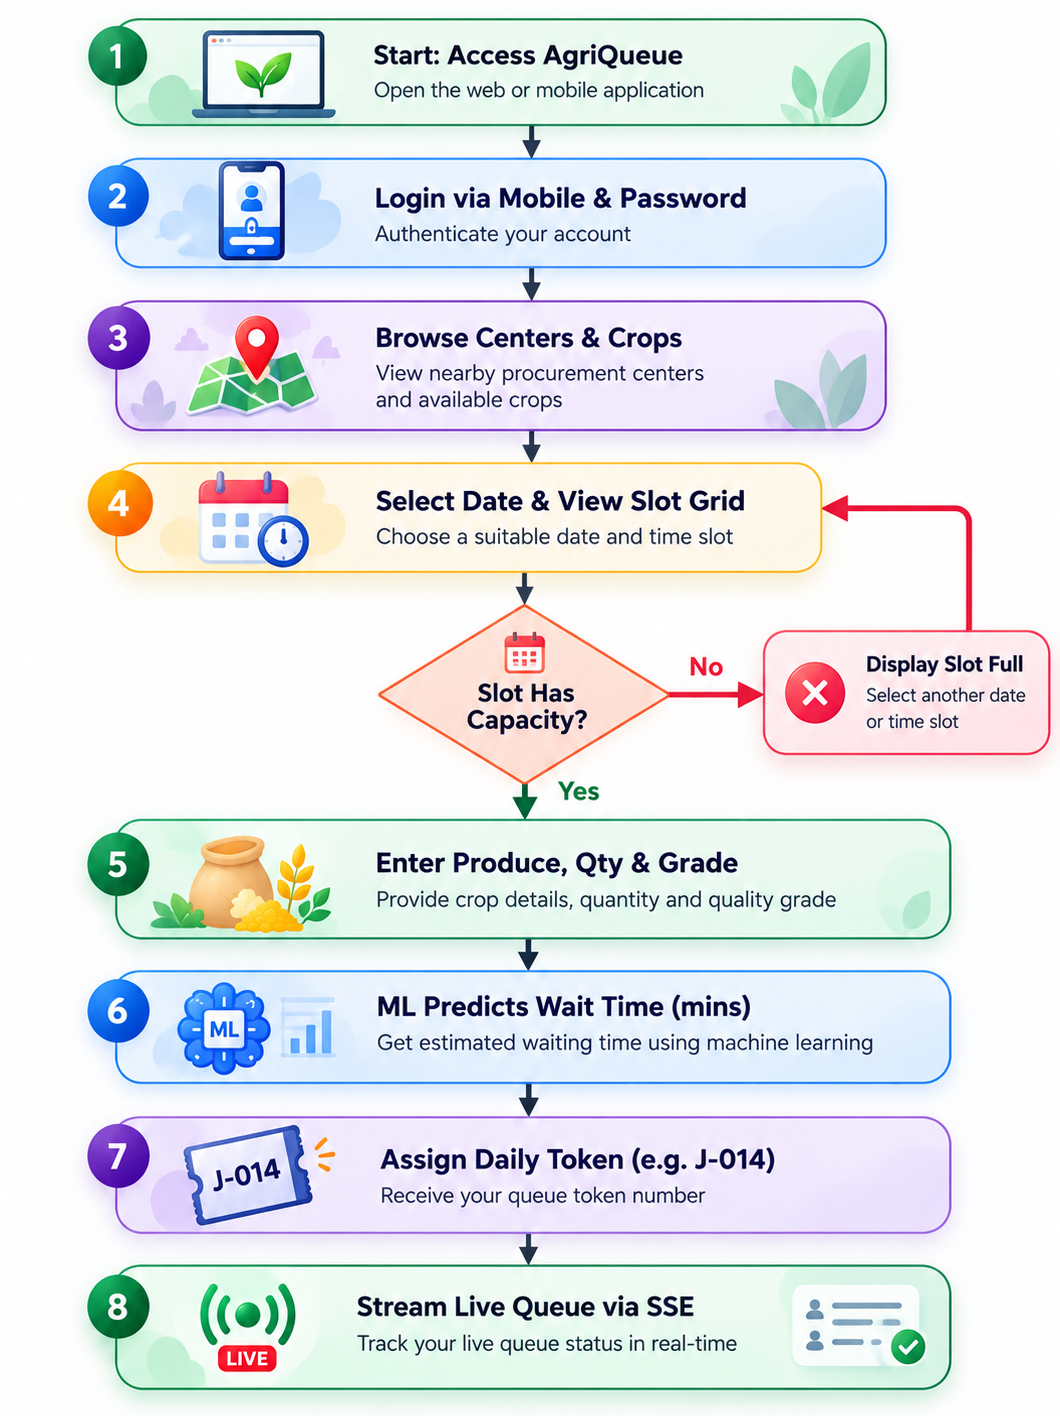
\includegraphics[width=0.58\textwidth]{img/flowchart_clean.png}
\caption{Farmer Slot Booking and Queue Progression Flowchart}
\label{fig:bookflow}
\end{figure}

\begin{itemize}
  \item \textbf{Capacity Validation:} Prevents overbooking by verifying that total booked quantity plus requested quantity remains within the slot threshold.
  \item \textbf{Predictive Estimation:} Invokes the HistGradientBoosting ML model with dynamic center features to display accurate wait expectations before the farmer departs home.
  \item \textbf{Token Sequencing:} Issues sequential per-center daily tokens guaranteeing deterministic service order upon physical arrival.
\end{itemize}

\newpage
\section{Staff Procurement Verification Flow}

The center operator utilizes an operational dashboard to systematically verify produce and issue payment records:

\begin{figure}[H]
\centering
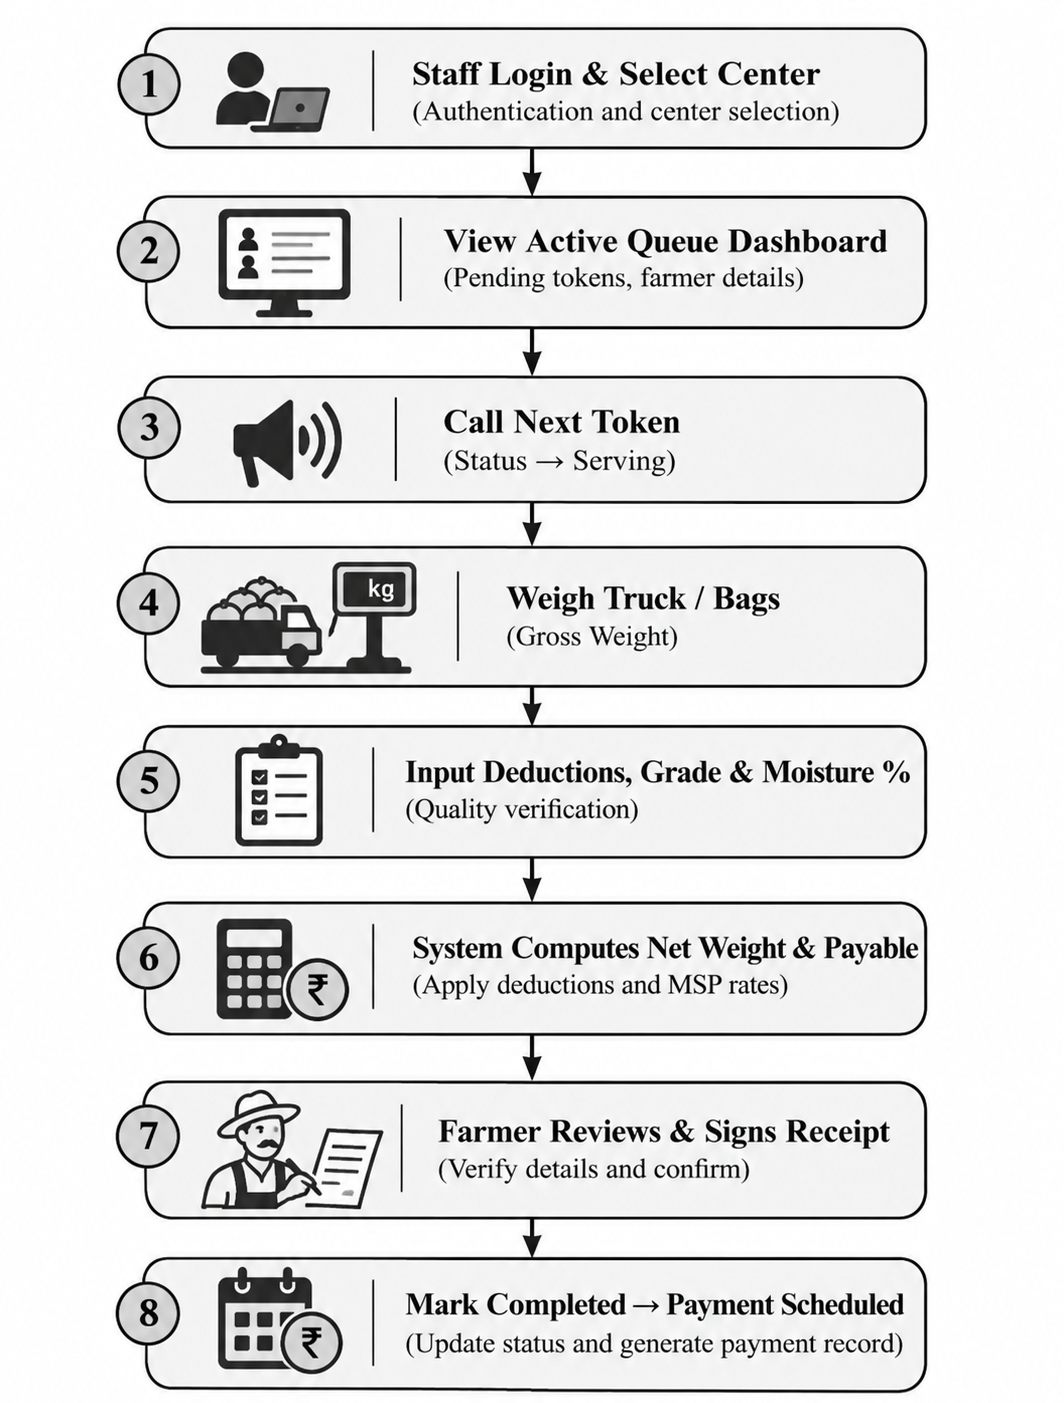
\includegraphics[width=0.58\textwidth]{img/staff_flow_clean.png}
\caption{Staff Procurement Physical Verification and Billing Flow}
\label{fig:staffflow}
\end{figure}

\begin{itemize}
  \item \textbf{Token Call Notification:} Updating a token to \textit{Serving} triggers immediate real-time SSE broadcasts and push notifications to the respective farmer.
  \item \textbf{Standardized Quality Grading:} Enforces standard government deduction tables for moisture content exceeding prescribed thresholds.
  \item \textbf{Automated Financial Calculations:} Eliminates manual math errors by programmatically evaluating:
  \begin{equation}
    \text{Net Weight} = \text{Actual Weight} - \text{Deductions}
  \end{equation}
  \begin{equation}
    \text{Net Payable} = \text{Net Weight} \times \text{Rate per kg}
  \end{equation}
\end{itemize}

\newpage
\section{System Interaction Sequence Diagrams}

System interactions across operational tiers and client boundaries are formalized below via three primary sequence workflows:

\subsection{Slot Booking and Predictive Wait-Time Allocation Sequence}

The booking sequence illustrates client validation, database slot capacity verification, scikit-learn machine learning wait estimation, and transactional token generation:

\begin{figure}[H]
\centering
\begin{tikzpicture}[
  header-client/.style={
    rectangle, draw=blue!85!black, fill=blue!15, rounded corners=5pt,
    text width=3.0cm, minimum height=0.9cm, align=center,
    font=\small\bfseries, line width=1.1pt, inner ysep=4pt
  },
  header-api/.style={
    rectangle, draw=blue!65!purple, fill=blue!12!purple!12, rounded corners=5pt,
    text width=3.0cm, minimum height=0.9cm, align=center,
    font=\small\bfseries, line width=1.1pt, inner ysep=4pt
  },
  header-ml/.style={
    rectangle, draw=purple!85!black, fill=purple!15, rounded corners=5pt,
    text width=3.0cm, minimum height=0.9cm, align=center,
    font=\small\bfseries, line width=1.1pt, inner ysep=4pt
  },
  header-db/.style={
    rectangle, draw=emerald!85!black, fill=emerald!16, rounded corners=5pt,
    text width=3.0cm, minimum height=0.9cm, align=center,
    font=\small\bfseries, line width=1.1pt, inner ysep=4pt
  },
  arr/.style={
    -{Latex[length=3.0mm, width=2.2mm]}, line width=1.3pt, draw=blue!85!black
  },
  ret/.style={
    -{Latex[length=3.0mm, width=2.2mm]}, dashed, line width=1.25pt, draw=purple!85!black
  },
  track/.style={
    draw=gray!65!black, line width=0.9pt, dash pattern=on 4pt off 3pt
  },
  lbl/.style={
    fill=white, inner sep=2pt, font=\scriptsize\bfseries, text=black
  }
]

% Lifelines (Columns at 1.6, 5.6, 9.6, 13.6)
\node[header-client] (C)  at (1.6, 8.4)  {Farmer Client\\(React SPA)};
\node[header-api]    (G)  at (5.6, 8.4)  {FastAPI Server\\(API Gateway)};
\node[header-ml]     (ML) at (9.6, 8.4)  {ML Engine\\(HistGBR)};
\node[header-db]     (DB) at (13.6, 8.4) {PostgreSQL DB\\(asyncpg)};

% Vertical Lifeline tracks
\draw[track] (C.south)  -- (1.6, 0.2);
\draw[track] (G.south)  -- (5.6, 0.2);
\draw[track] (ML.south) -- (9.6, 0.2);
\draw[track] (DB.south) -- (13.6, 0.2);

% Messages
\draw[arr] (1.6, 6.9) -- node[lbl, above=1pt]{1: GET /centers/\{id\}/slots?date=...} (5.6, 6.9);
\draw[arr] (5.6, 6.2) -- node[lbl, above=1pt]{2: SELECT capacity, booked\_kg FROM slots} (13.6, 6.2);
\draw[ret] (13.6, 5.5) -- node[lbl, above=1pt]{3: Return available quotas per slot} (5.6, 5.5);
\draw[ret] (5.6, 4.8) -- node[lbl, above=1pt]{4: HTTP 200: Slot availability grid} (1.6, 4.8);

\draw[arr] (1.6, 4.0) -- node[lbl, above=1pt]{5: POST /bookings \{crop, qty\_kg, slot\_id\}} (5.6, 4.0);
\draw[arr] (5.6, 3.3) -- node[lbl, above=1pt]{6: predict(13 center \& queue features)} (9.6, 3.3);
\draw[ret] (9.6, 2.6) -- node[lbl, above=1pt]{7: Return wait = 38 min, range [34, 42]} (5.6, 2.6);

\draw[arr] (5.6, 1.8) -- node[lbl, above=1pt]{8: INSERT INTO bookings \& assign next token} (13.6, 1.8);
\draw[ret] (13.6, 1.1) -- node[lbl, above=1pt]{9: COMMIT (Token = J-014, ID = 108)} (5.6, 1.1);
\draw[ret] (5.6, 0.4) -- node[lbl, above=1pt]{10: HTTP 201: \{Token: J-014, EstWait: 38 min\}} (1.6, 0.4);

\end{tikzpicture}
\caption{End-to-End Slot Booking and ML Wait-Time Prediction Sequence Diagram}
\label{fig:seq-booking}
\end{figure}

\subsection{Physical Procurement Weighment and Payment Settlement Sequence}

The procurement intake workflow coordinates center scales, moisture quality grading, government MSP evaluation, and automated digital disbursement creation:

\begin{figure}[H]
\centering
\begin{tikzpicture}[
  header-staff/.style={
    rectangle, draw=teal!90!black, fill=teal!16, rounded corners=5pt,
    text width=3.0cm, minimum height=0.9cm, align=center,
    font=\small\bfseries, line width=1.1pt, inner ysep=4pt
  },
  header-api/.style={
    rectangle, draw=cyan!85!black, fill=cyan!15, rounded corners=5pt,
    text width=3.0cm, minimum height=0.9cm, align=center,
    font=\small\bfseries, line width=1.1pt, inner ysep=4pt
  },
  header-db/.style={
    rectangle, draw=emerald!90!black, fill=emerald!16, rounded corners=5pt,
    text width=3.0cm, minimum height=0.9cm, align=center,
    font=\small\bfseries, line width=1.1pt, inner ysep=4pt
  },
  header-farmer/.style={
    rectangle, draw=blue!85!black, fill=blue!15, rounded corners=5pt,
    text width=3.0cm, minimum height=0.9cm, align=center,
    font=\small\bfseries, line width=1.1pt, inner ysep=4pt
  },
  arr/.style={
    -{Latex[length=3.0mm, width=2.2mm]}, line width=1.3pt, draw=teal!90!black
  },
  arr-blue/.style={
    -{Latex[length=3.0mm, width=2.2mm]}, line width=1.3pt, draw=blue!85!black
  },
  ret/.style={
    -{Latex[length=3.0mm, width=2.2mm]}, dashed, line width=1.25pt, draw=purple!85!black
  },
  track/.style={
    draw=gray!65!black, line width=0.9pt, dash pattern=on 4pt off 3pt
  },
  lbl/.style={
    fill=white, inner sep=2pt, font=\scriptsize\bfseries, text=black
  }
]

% Lifelines (Columns at 1.6, 5.6, 9.6, 13.6)
\node[header-staff]  (S)   at (1.6, 8.4)  {Center Staff\\(Operator UI)};
\node[header-api]    (API) at (5.6, 8.4)  {FastAPI Server\\(Procurement)};
\node[header-db]     (DB)  at (9.6, 8.4)  {PostgreSQL DB\\(Relational)};
\node[header-farmer] (F)   at (13.6, 8.4) {Farmer Client\\(SSE / WebPush)};

% Vertical Lifeline tracks
\draw[track] (S.south)   -- (1.6, 0.2);
\draw[track] (API.south) -- (5.6, 0.2);
\draw[track] (DB.south)  -- (9.6, 0.2);
\draw[track] (F.south)   -- (13.6, 0.2);

% Messages
\draw[arr] (1.6, 6.9) -- node[lbl, above=1pt]{1: POST /queue/call-next \{token: J-014\}} (5.6, 6.9);
\draw[arr] (5.6, 6.2) -- node[lbl, above=1pt]{2: UPDATE bookings SET status = 'Serving'} (9.6, 6.2);
\draw[arr-blue] (5.6, 5.5) -- node[lbl, above=1pt]{3: SSE Broadcast: "Now Serving Token J-014"} (13.6, 5.5);

\draw[arr] (1.6, 4.6) -- node[lbl, above=1pt]{4: Input physical scale weight \& moisture \%} (5.6, 4.6);
\draw[arr] (5.6, 3.9) -- node[lbl, above=1pt]{5: SELECT msp\_rate FROM produces} (9.6, 3.9);
\draw[ret] (9.6, 3.2) -- node[lbl, above=1pt]{6: Return MSP rate (e.g. Rs. 24/kg)} (5.6, 3.2);

\draw[ret] (5.6, 2.5) -- node[lbl, above=1pt]{7: Return Net Wt: 1,000kg \& Payable: Rs. 24,000} (1.6, 2.5);
\draw[arr] (1.6, 1.8) -- node[lbl, above=1pt]{8: POST /procurement/complete (Confirm bill)} (5.6, 1.8);
\draw[arr] (5.6, 1.1) -- node[lbl, above=1pt]{9: INSERT INTO records \& payments (Scheduled)} (9.6, 1.1);
\draw[arr-blue] (5.6, 0.4) -- node[lbl, above=1pt]{10: VAPID Push Alert: Digital Receipt \#RCP-0491} (13.6, 0.4);

\end{tikzpicture}
\caption{Physical Procurement Weighment and Digital Payment Settlement Sequence Diagram}
\label{fig:seq-procurement}
\end{figure}

\subsection{Real-Time Live Queue SSE Synchronization Sequence}

Server-Sent Events provide a persistent, single-direction HTTP connection enabling sub-second synchronization between physical center operations and farmer devices:

\begin{figure}[H]
\centering
\begin{tikzpicture}[
  header-client/.style={
    rectangle, draw=blue!85!black, fill=blue!15, rounded corners=5pt,
    text width=3.4cm, minimum height=0.9cm, align=center,
    font=\small\bfseries, line width=1.1pt, inner ysep=4pt
  },
  header-server/.style={
    rectangle, draw=teal!90!black, fill=teal!16, rounded corners=5pt,
    text width=3.4cm, minimum height=0.9cm, align=center,
    font=\small\bfseries, line width=1.1pt, inner ysep=4pt
  },
  header-db/.style={
    rectangle, draw=emerald!90!black, fill=emerald!16, rounded corners=5pt,
    text width=3.4cm, minimum height=0.9cm, align=center,
    font=\small\bfseries, line width=1.1pt, inner ysep=4pt
  },
  arr/.style={
    -{Latex[length=3.0mm, width=2.2mm]}, line width=1.3pt, draw=blue!85!black
  },
  ret/.style={
    -{Latex[length=3.0mm, width=2.2mm]}, dashed, line width=1.25pt, draw=purple!85!black
  },
  track/.style={
    draw=gray!65!black, line width=0.9pt, dash pattern=on 4pt off 3pt
  },
  lbl/.style={
    fill=white, inner sep=2pt, font=\scriptsize\bfseries, text=black
  }
]

% Lifelines (Columns at 2.0, 7.6, 13.2)
\node[header-client] (C) at (2.0, 8.0)  {Farmer Client\\(Browser / Mobile)};
\node[header-server] (S) at (7.6, 8.0)  {FastAPI Server\\(SSE Event Stream)};
\node[header-db]     (D) at (13.2, 8.0) {PostgreSQL DB\\(Active Session)};

% Vertical Lifeline tracks
\draw[track] (C.south) -- (2.0, 0.1);
\draw[track] (S.south) -- (7.6, 0.1);
\draw[track] (D.south) -- (13.2, 0.1);

% Messages
\draw[arr] (2.0, 6.4) -- node[lbl, above=1pt]{1: GET /queue/\{center\_id\}/stream (Establish SSE Connection)} (7.6, 6.4);
\draw[arr] (7.6, 5.2) -- node[lbl, above=1pt]{2: SELECT active bookings for today} (13.2, 5.2);
\draw[ret] (13.2, 4.0) -- node[lbl, above=1pt]{3: Return sorted queue rows (Token, Status)} (7.6, 4.0);

% In-server processing box
\node[rectangle, draw=teal!90!black, fill=teal!14, rounded corners=5pt,
      text width=5.2cm, minimum height=0.74cm, align=center,
      font=\scriptsize\bfseries, text=teal!95!black, line width=1.1pt] at (7.6, 2.7)
      {4: Compute tokens ahead \& ML wait estimation};

\draw[arr] (7.6, 1.5) -- node[lbl, above=1pt]{5: data: \{serving: 5, your\_token: 7, wait: 14\}} (2.0, 1.5);

% Periodic loop indication
\node[rectangle, draw=amber!90!black, dashed, fill=amber!14, rounded corners=5pt,
      text width=11.6cm, minimum height=0.74cm, align=center,
      font=\scriptsize\bfseries, text=amber!95!black, line width=1.1pt] at (7.6, 0.5)
      {\textbf{Active SSE Polling Loop:} Steps 2 through 5 automatically re-execute every 5 seconds};

\end{tikzpicture}
\caption{Server-Sent Events (SSE) Live Queue Sequence Diagram}
\label{fig:sse}
\end{figure}

\begin{itemize}
  \item \textbf{Low Overhead:} Compared to WebSocket handshakes, SSE operates over standard HTTP/1.1 or HTTP/2, requiring no specialized proxy configuration.
  \item \textbf{Fresh Database Sessions:} Each 5-second polling cycle allocates an independent scoped database transaction, avoiding stale object references or connection leaks.
  \item \textbf{Graceful Disconnect Handling:} Client network interruptions trigger automatic browser-managed reconnect backoffs with zero server-side zombie processes.
\end{itemize}

\section{Cloud Deployment Topology}

The production infrastructure combines serverless edge hosting with containerized backend services:

\begin{figure}[H]
\centering
\begin{tikzpicture}[
  tier/.style={rectangle, draw=gray!70!black, fill=gray!8, rounded corners=5pt,
               text width=2.8cm, minimum height=0.85cm, align=center, font=\scriptsize\bfseries},
  arr/.style={->, >=Latex, thick, draw=gray!70!black},
  lbl/.style={fill=white, inner sep=2pt, font=\tiny\bfseries, text=gray!80!black}
]

% Topology Nodes
\node[tier, fill=blue!10]   (CL)  at (0, 2.5)   {Client Layer\\(Mobile / PC / Tab)};
\node[tier, fill=purple!10] (CDN) at (5.2, 4.3) {Vercel Edge CDN\\(React 19 Frontend)};
\node[tier, fill=teal!10]   (API) at (5.2, 0.7) {Cloud VPS Server\\(FastAPI + Uvicorn)};
\node[tier, fill=amber!15]  (EXT) at (10.4, 4.3){External Services\\(WebPush + Gemini)};
\node[tier, fill=orange!12] (DB)  at (10.4, 0.7){Managed Cloud DB\\(PostgreSQL 15)};

% 1. Client to CDN (North-east orthogonal)
\draw[arr] (CL.north) -- ++(0, 1.2) -| (CDN.west) node[pos=0.25, lbl]{HTTPS (Assets)};

% 2. Client to Backend API (South-east orthogonal)
\draw[arr] (CL.south) -- ++(0, -1.2) -| (API.west) node[pos=0.25, lbl]{HTTPS / SSE};

% 3. Backend to PostgreSQL (Straight horizontal)
\draw[arr] (API.east) -- (DB.west) node[midway, lbl]{asyncpg + TLS};

% 4. Backend to External Services (Clean orthogonal between columns)
\draw[arr] (API.north east) -- ++(1.0, 0.6) |- (EXT.south west) node[pos=0.4, lbl]{VAPID / REST};

% 5. External Services to Client (Overhead loop)
\draw[arr] (EXT.north) -- ++(0, 0.9) -| (CL.north west) node[pos=0.25, lbl]{Push Notification (VAPID)};

\end{tikzpicture}
\caption{Production Cloud Deployment Topology}
\label{fig:deploy}
\end{figure}

\begin{itemize}
  \item \textbf{Vercel CDN Edge:} Serves immutable static bundles with aggressive global caching, reducing frontend latency to $<$50ms.
  \item \textbf{FastAPI Application Server:} Hosted on Ubuntu cloud instance with automatic restart policies and TLS encryption for all incoming and outgoing connections.
  \item \textbf{PostgreSQL Relational DB:} Enforces automated daily backups, read-write query optimization, and persistent volume encryption.
\end{itemize}

\section{System Functional Modules}

AgriQueue is partitioned into ten distinct functional subsystems:
\begin{itemize}
  \item \textbf{M1: Authentication \& Role-Based Access Control (RBAC):} Secure HTTP-only JWT cookie management with Argon2id password hashing across Farmer, Staff, and Admin roles.
  \item \textbf{M2: Center Discovery \& Slot Scheduling:} Configurable daily operational windows, crop acceptance rules, and automated capacity counting per time block.
  \item \textbf{M3: Booking Lifecycle Engine:} Capacity enforcement, token generation, wait-time prediction linkage, and policy-governed cancellations.
  \item \textbf{M4: Real-Time SSE Queue Streamer:} Asynchronous event emitter providing sub-5-second queue positioning updates to active farmer sessions.
  \item \textbf{M5: Machine Learning Wait Time Predictor:} HistGradientBoosting regression model trained on 10,000 historical queue observations ($R^2 = 0.988$).
  \item \textbf{M6: Staff Procurement Verification:} Physical weighment intake, automated quality grading deductions, and net payable calculation.
  \item \textbf{M7: Digital Payment Lifecycle:} Automated transition from Scheduled $\to$ Processing $\to$ Settled, backed by audit logs and farmer dispute management.
  \item \textbf{M8: Administrative Control Center:} Complete administrative CRUD interfaces for centers, slots, crops, pricing schedules, and staff rosters.
  \item \textbf{M9: Web Push Notification Dispatcher:} Standards-compliant VAPID push alerts delivered directly to mobile browsers for queue turns and payments.
  \item \textbf{M10: AI Command Assistant:} LangGraph ReAct agent powered by Google Gemini for natural language system querying and reporting.
\end{itemize}
